% 内积空间：Gram矩阵（正定与半正定、加权内积、Gram因子、逐元素乘积、基的Gram矩阵、复情形）。

\section{Gram矩阵}
\label{sec:ls-gram-psd}

一组向量的全部两两内积可以排成一个对称矩阵，即Gram矩阵。本节先引入正定与半正定矩阵，并用正定矩阵定义$\mathbb R^d$上的加权内积；然后定义Gram矩阵，说明Gram矩阵恰好是全部半正定矩阵，从中可以读出这组向量是否线性无关、是否两两正交。借助这一刻画，可以证明逐元素乘积保持半正定。最后用基的Gram矩阵写出一般内积在坐标下的计算公式。

\subsection{正定与半正定}
\label{sec:ls-positive-definite}
$n$阶对称矩阵$\bm M$与向量$\bm x\in\mathbb R^n$给出一个数
\[
 q(\bm x)=\sum_{i=1}^n\sum_{j=1}^n m_{i,j}x_ix_j,
\]
称为$\bm M$的二次型；用矩阵乘法，它写作$\bm x^\top\bm M\bm x$。

若对每个非零$\bm x$都有$q(\bm x)>0$，就称$\bm M$\term{正定}（positive definite），记作$\bm M\succ\bm0$；若只保证$q(\bm x)\geq0$对一切$\bm x$成立，就称$\bm M$\term{半正定}（positive semidefinite），记作$\bm M\succeq\bm0$。

对两个同阶对称矩阵，$\bm M\succeq\bm N$表示$\bm M-\bm N\succeq\bm0$，即$\bm M$的二次型处处不小于$\bm N$的二次型。它比较的是两个二次型，不是逐个元素。

判断正定性，要看二次型能否在某个非零向量处取到零或负值。下面用配方比较两个二阶矩阵。
\begin{example}[用配方区分正定与半正定]
\label{ex:ls-pd-psd-completing-square}
比较
\[
 \bm M=\begin{bmatrix}4&2\\2&2\end{bmatrix},\quad
 \bm N=\begin{bmatrix}1&1\\1&1\end{bmatrix}.
\]
把二次型配成平方和，非负性一目了然，剩下的问题是平方和能否在非零向量处为零：
\[
 \begin{aligned}
 q_{\bm M}(\bm x)&=4x_1^2+4x_1x_2+2x_2^2=(2x_1+x_2)^2+x_2^2,\\
 q_{\bm N}(\bm x)&=x_1^2+2x_1x_2+x_2^2=(x_1+x_2)^2.
 \end{aligned}
\]
$q_{\bm M}$是两个平方之和，只在$2x_1+x_2=0$且$x_2=0$，即$\bm x=\bm0$时为零，所以$\bm M\succ\bm0$。$q_{\bm N}$只有一个平方，它处处非负，却在非零向量$\bm x=(1,-1)^\top$处为零，所以$\bm N\succeq\bm0$而不是正定矩阵。两个变量的二次型配出两个独立的平方项时正定，只配出一个平方项时半正定而不正定。
\end{example}

对角矩阵的情形最简单。它的二次型是$\sum_id_ix_i^2$。若全部$d_i>0$，每个非零$\bm x$都使它为正；若某个$d_i\leq0$，取$\bm x=\bm e_i$就得到$q(\bm e_i)=d_i\leq0$。所以对角矩阵正定当且仅当全部$d_i>0$，例如$\bm I_n\succ\bm0$。

一般矩阵的正定性要对全部非零向量检查，只看元素的符号并不够。
\begin{example}[反例：元素全为正的对称矩阵未必正定]
\label{ex:ls-positive-entries-not-pd}
矩阵
\[
 \bm M=\begin{bmatrix}1&2\\2&1\end{bmatrix}
\]
的四个元素都为正，二次型为$q(\bm x)=x_1^2+4x_1x_2+x_2^2$。交叉项系数比两个平方项大，只要让$x_1,x_2$异号，交叉项就会占上风。取$\bm x=(1,-1)^\top$，
\[
 q(\bm x)=1^2+4\cdot1\cdot(-1)+(-1)^2=-2<0,
\]
所以$\bm M$不是正定矩阵，连半正定也不是。决定正定性的是二次型在所有方向上的取值，而不是元素的符号。
\end{example}

\paragraph{加权内积}
\phantomsection
\label{sec:ls-weighted-inner-products}
正定矩阵可以用来在$\mathbb R^d$上定义标准内积以外的内积。各坐标的单位或重要性不同时，可以给不同方向不同的权重：取对称正定矩阵$\bm M$，规定
\begin{equation}
\begin{gathered}
\langle\bm x,\bm y\rangle_{\bm M}=\bm x^\top\bm M\bm y,\\
d_{\bm M}(\bm x,\bm y)=\lVert\bm x-\bm y\rVert_{\bm M}=\sqrt{(\bm x-\bm y)^\top\bm M(\bm x-\bm y)}.
\end{gathered}
\label{eq:linear-algebra-mahalanobis-pseudodistance}
\end{equation}
双线性来自矩阵乘法的分配律，对称性来自$\bm M^\top=\bm M$，正定性就是$\bm M$的正定性。所以它满足内积的三条公理，称为加权内积，$d_{\bm M}$是它给出的距离。统计中取$\bm M$为协方差矩阵的逆，得到的就是Mahalanobis距离。下面看权重怎样改变同一个点的长度。
\begin{example}[加权内积下的长度]
\label{ex:ls-weighted-length}
取$\bm M=\operatorname{diag}(4,1)$，加权内积就是$\langle\bm x,\bm y\rangle_{\bm M}=4x_1y_1+x_2y_2$，第一个坐标的乘积被计为四倍。对点$\bm x=(1,1)^\top$，$\lVert\bm x\rVert_{\bm M}^2=4\cdot1+1\cdot1=5$，而欧氏长度的平方只有$1+1=2$。同一个点的加权长度是$\sqrt5$，欧氏长度是$\sqrt2$：权重放大了第一个坐标对长度的贡献，第一个坐标上的偏差因而比第二个坐标上同样大小的偏差显得更远。
\end{example}
本节最后将说明，选定基以后，任一实内积都可以写成这种加权形式。

\subsection{Gram矩阵的定义}
\label{sec:ls-gram-orthogonality}
正交是两个向量之间的关系。一组向量$\bm b_1,\ldots,\bm b_r$之间有$r^2$个内积值，把它们排成一个矩阵，就能一次记录这组向量的全部相互关系。
\begin{definition}[有限向量族的Gram矩阵]
\label{def:linear-algebra-gram-matrix}
设$\bm b_1,\ldots,\bm b_r$是内积空间$V$中的向量。以$g_{i,j}=\langle\bm b_i,\bm b_j\rangle$为元素的$r$阶矩阵$\bm G$称为它们的\term{Gram矩阵}（Gram matrix）。在$\mathbb R^m$中，若$\bm B$以这些向量为列，则欧氏内积下$\bm G=\bm B^\top\bm B$，加权内积$\langle\cdot,\cdot\rangle_{\bm M}$下$\bm G=\bm B^\top\bm M\bm B$。
\end{definition}
矩阵形式来自乘积的元素公式：$(\bm B^\top\bm B)_{i,j}$是$\bm B^\top$的第$i$行（即$\bm b_i^\top$）与$\bm B$的第$j$列相乘。由内积的对称性，$\bm G$是对称矩阵。

正交性写在Gram矩阵的非对角元里：$\bm G$是对角矩阵，恰好表示这组向量两两正交；$\bm G=\bm I_r$，则表示它们两两正交且长度都为$1$。图~\ref{fig:ls-gram-matrix-coefficients}把两个向量的两两内积排成数表。
\begin{figure}[!htb]
  \centering
  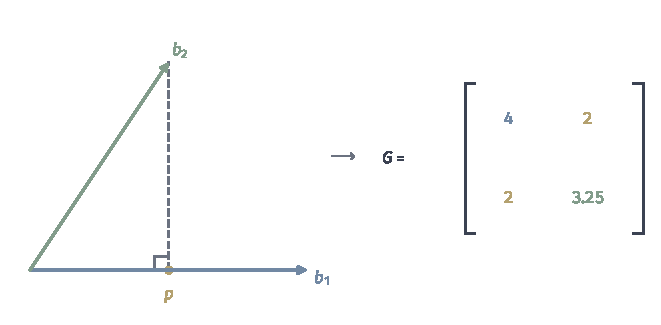
\includegraphics[width=112mm]{figures/00-shared/mathematical-preliminaries-upper/02-linear-spaces/matplotlib/ls-gram-matrix-coefficients/ls-gram-matrix-coefficients.pdf}
  \caption{Gram矩阵把一组基向量的两两内积排成数表。左：平面上两条不垂直的基向量$\bm b_1,\bm b_2$及其夹角；右：$G_{i,j}=\langle\bm b_i,\bm b_j\rangle$构成的$2\times2$Gram矩阵，对角元为各向量长度的平方，非对角元为两向量的内积。基越接近正交，非对角元越接近零；两向量共线时，某个非零组合的平方长度为零，Gram矩阵不再正定。向量与矩阵均为解析教学例。}
  \label{fig:ls-gram-matrix-coefficients}
\end{figure}

\subsection{Gram矩阵与半正定矩阵}
\label{sec:ls-gram-semidefinite}

\paragraph{Gram矩阵的半正定性}
Gram矩阵的二次型就是线性组合的长度平方。对任意系数向量$\bm a\in\mathbb R^r$，按双线性展开得
\[
 \bm a^\top\bm G\bm a=\sum_{i,j}a_ia_j\langle\bm b_i,\bm b_j\rangle=\Bigl\lVert\sum_j a_j\bm b_j\Bigr\rVert^2\geq0,
\]
所以Gram矩阵半正定。

Gram矩阵正定，当且仅当只有全零系数使线性组合$\sum_ja_j\bm b_j$为零，即这组向量线性无关（第~\ref{sec:ls-linear-dependence}节）：组合为零时平方长度为零，组合非零时平方长度为正。正定的Gram矩阵可逆：若$\bm G\bm a=\bm0$，则$\bm a^\top\bm G\bm a=0$，从而$\bm a=\bm0$，零空间为零（第~\ref{sec:ls-injective-surjective-invertible}节）。

近共线在Gram矩阵上也有对应的表现。
\begin{example}[近共线两列的Gram矩阵]
\label{ex:ls-nearly-collinear-gram}
仍取贯穿例的两列$\bm c_1,\bm c_2$与欧氏内积。示例~\ref{ex:ls-nearly-collinear-angle}已经算出三个内积，把它们排成矩阵，再写出二次型：
\[
\begin{gathered}
\bm G=\bm X_\varepsilon^\top\bm X_\varepsilon=\begin{bmatrix}3&3\\3&3+2\varepsilon^2\end{bmatrix},\\
\bm a^\top\bm G\bm a=3(a_1+a_2)^2+2\varepsilon^2a_2^2 .
\end{gathered}
\]
$\varepsilon\neq0$时，二次型只在$a_1=a_2=0$时为零，所以$\bm G$正定，这与两列线性无关一致。但正定的余量很小：取$\bm a=(1,-1)^\top$，第一个平方项消失，二次型只剩$2\varepsilon^2$；对应的组合$\bm c_1-\bm c_2=-\varepsilon\bm q$确实很短。近共线在Gram矩阵上的表现就是“正定但几乎退化”：系数不全为零，线性组合的长度平方却可以接近零。
\end{example}

\paragraph{Gram因子定理}
Gram矩阵总是半正定的。反过来，每个半正定矩阵是否都是某组向量的Gram矩阵？关键是把半正定矩阵的二次型写成欧氏平方和。下面的定理用逐步配方给出这一分解。
\begin{theorem}[半正定矩阵的配方因子]
\label{thm:ls-gram-factor}
设$\bm M\in\mathbb R^{r\times r}$对称半正定，则存在$\bm L\in\mathbb R^{r\times r}$使$\bm M=\bm L^\top\bm L$；若$\bm M$正定，可取$\bm L$可逆。
\end{theorem}
\begin{proof}
对$r$归纳。$r=1$时$\bm M=(m_{1,1})$且$m_{1,1}\geq0$，取$\bm L=(\sqrt{m_{1,1}})$即可。

设$r>1$。若所有对角元都为零，任取$i\neq j$，把$\bm x=\bm e_i+t\bm e_j$代入半正定性：
\[
 0\leq\bm x^\top\bm M\bm x=m_{i,i}+2t\,m_{i,j}+t^2m_{j,j}=2t\,m_{i,j}.
\]
这对正负$t$同时成立，迫使$m_{i,j}=0$，于是$\bm M=\bm0$，取$\bm L=\bm0$。

否则存在正的对角元。取一个置换矩阵$\bm P$把它换到首位（行列同步交换）；$\bm P$的各列是互不相同的标准坐标向量，所以$\bm P^\top\bm P=\bm P\bm P^\top=\bm I$。记
\[
\begin{gathered}
\widetilde{\bm M}=\bm P\bm M\bm P^\top
 =\begin{bmatrix}a&\bm b^\top\\ \bm b&\bm C\end{bmatrix},\\
a>0.
\end{gathered}
\]
$\widetilde{\bm M}$仍对称半正定，因为$\bm x^\top\widetilde{\bm M}\bm x=(\bm P^\top\bm x)^\top\bm M(\bm P^\top\bm x)\geq0$。对第一个变量配方：令$\bm x=(-\bm b^\top\bm u/a,\bm u)$，展开得$\bm x^\top\widetilde{\bm M}\bm x=\bm u^\top(\bm C-\bm b\bm b^\top/a)\bm u\geq0$，故余项$\bm M'=\bm C-\bm b\bm b^\top/a$仍半正定。由归纳假设$\bm M'=\bm L'^\top\bm L'$，取上三角因子
\[
 \widetilde{\bm L}=\begin{bmatrix}\sqrt a&\bm b^\top/\sqrt a\\ \bm0&\bm L'\end{bmatrix},
\]
按分块乘法直接相乘得
\[
 \widetilde{\bm L}^\top\widetilde{\bm L}
 =\begin{bmatrix}a&\bm b^\top\\ \bm b&\bm b\bm b^\top/a+\bm L'^\top\bm L'\end{bmatrix}
 =\widetilde{\bm M}.
\]
换回原矩阵：$\bm M=\bm P^\top\widetilde{\bm M}\bm P=(\widetilde{\bm L}\bm P)^\top(\widetilde{\bm L}\bm P)$，取$\bm L=\widetilde{\bm L}\bm P$即可。

正定时，$\bm M'$也正定（上述$\bm x$在$\bm u\neq\bm0$时非零），由归纳假设$\bm L'$可逆。分块上三角矩阵$\widetilde{\bm L}$的对角块$\sqrt a$与$\bm L'$都可逆，按分块乘法可以直接验证
\[
 \begin{bmatrix}1/\sqrt a&-\bm b^\top\bm L'^{-1}/a\\ \bm0&\bm L'^{-1}\end{bmatrix}
\]
是它的逆。于是$\bm L=\widetilde{\bm L}\bm P$作为可逆矩阵的乘积仍可逆。
\end{proof}
下面对一个二阶正定矩阵按证明的步骤求出因子。
\begin{example}[二阶正定矩阵的配方因子]
\label{ex:ls-gram-factor-two-by-two}
取示例~\ref{ex:ls-pd-psd-completing-square}中的正定矩阵
\[
 \bm M=\begin{bmatrix}4&2\\2&2\end{bmatrix}.
\]
首个对角元$a=4>0$，不需要置换。分块后$\bm b=(2)$，配方剩下的余项是$\bm M'=2-2^2/4=1$，它是一阶矩阵，取$\bm L'=(1)$。代入证明中的分块形式，
\[
 \bm L=\begin{bmatrix}\sqrt a&\bm b^\top/\sqrt a\\ 0&\bm L'\end{bmatrix}=\begin{bmatrix}2&1\\0&1\end{bmatrix}.
\]
相乘即可验证：
\[
 \bm L^\top\bm L=\begin{bmatrix}2&0\\1&1\end{bmatrix}\begin{bmatrix}2&1\\0&1\end{bmatrix}=\begin{bmatrix}4&2\\2&2\end{bmatrix}=\bm M.
\]
$\bm L$是对角元为正的上三角矩阵，因而可逆。它的两行正是配方中两个平方项的系数：
\[
 \bm x^\top\bm M\bm x=4x_1^2+4x_1x_2+2x_2^2=(2x_1+x_2)^2+x_2^2 ,
\]
即$\bm x^\top\bm M\bm x=\lVert\bm L\bm x\rVert_2^2$。证明中的分块步骤与手工配方是同一件事。
\end{example}
由这个分解，正定矩阵给出的加权长度可写成$\lVert\bm x\rVert_{\bm M}=\lVert\bm L\bm x\rVert_2$：加权内积就是把$\bm x$换成新坐标$\bm L\bm x$后再量欧氏长度。证明中的配方步骤就是第~\ref{sec:ls-cholesky}节Cholesky分解的雏形。

\paragraph{半正定矩阵是Gram矩阵}
因子定理回答了上面的问题：每个半正定矩阵都是某组向量的Gram矩阵。由定理~\ref{thm:ls-gram-factor}，半正定的$\bm M$可写成$\bm M=\bm L^\top\bm L$。记$\bm l_i$为$\bm L$的第$i$列，则$m_{i,j}=\bm l_i^\top\bm l_j=\langle\bm l_i,\bm l_j\rangle$，所以$\bm M$正是$\bm l_1,\ldots,\bm l_r$在欧氏内积下的Gram矩阵。于是“半正定”与“是一组向量的两两内积”说的是同一件事；要判断一个矩阵半正定，可以去找这样一组向量。

\subsection{Gram矩阵的逐元素乘法}
\label{sec:ls-schur-product}
利用“半正定矩阵就是Gram矩阵”这一刻画，可以判断两个半正定矩阵的逐元素乘积（第~\ref{sec:ls-hadamard-product}节）是否仍然半正定。

两个半正定矩阵分别是两组向量的Gram矩阵；只要再找到一组向量，使它们的两两内积恰为两个Gram矩阵对应元素之积，就能断定乘积半正定。所得结论称为\term{Schur乘积}定理（Schur product theorem）。
\begin{theorem}[Schur乘积定理]
\label{thm:ls-schur-product}
设$\bm A,\bm B$均为$n$阶对称半正定矩阵，则逐元素乘积$\bm A\odot\bm B$也对称半正定。
\end{theorem}
\begin{proof}
对称性由$(\bm A\odot\bm B)_{k,i}=A_{k,i}B_{k,i}=A_{i,k}B_{i,k}$直接得到。由定理~\ref{thm:ls-gram-factor}，$\bm A=\bm U^\top\bm U$、$\bm B=\bm V^\top\bm V$；记$\bm u_i,\bm v_i$分别为$\bm U,\bm V$的第$i$列，则$A_{i,k}=\langle\bm u_i,\bm u_k\rangle$、$B_{i,k}=\langle\bm v_i,\bm v_k\rangle$。考虑二阶数组$\bm u_1\otimes\bm v_1,\ldots,\bm u_n\otimes\bm v_n$。由Frobenius内积下张量积配对的分离性（第~\ref{sec:ls-tensor-product-properties}节），它们的Gram矩阵为
\[
 \langle\bm u_i\otimes\bm v_i,\bm u_k\otimes\bm v_k\rangle_{\mathrm F}
 =\langle\bm u_i,\bm u_k\rangle\langle\bm v_i,\bm v_k\rangle
 =A_{i,k}B_{i,k}.
\]
所以$\bm A\odot\bm B$是$\bm u_1\otimes\bm v_1,\ldots,\bm u_n\otimes\bm v_n$的Gram矩阵；Gram矩阵恒半正定，故$\bm A\odot\bm B$半正定。
\end{proof}
下面用一个二阶例子核对。
\begin{example}[两个半正定矩阵的逐元素乘积]
\label{ex:ls-schur-product}
取
\[
 \bm A=\bm B=\begin{bmatrix}1&1\\1&2\end{bmatrix}.
\]
先确认前提：$\bm A$的二次型为$x_1^2+2x_1x_2+2x_2^2=(x_1+x_2)^2+x_2^2\geq0$，所以$\bm A$半正定。逐元素相乘只把对角元$2$变成$4$，乘积及其二次型为
\[
\begin{gathered}
\bm A\odot\bm B=\begin{bmatrix}1&1\\1&4\end{bmatrix},\\
x_1^2+2x_1x_2+4x_2^2=(x_1+x_2)^2+3x_2^2\geq0 .
\end{gathered}
\]
配方后仍是平方和，$\bm A\odot\bm B$半正定，与定理~\ref{thm:ls-schur-product}一致。这里的配方只是核对；定理的作用在于，不必对每个乘积重新配方，就能断定结果半正定。
\end{example}
核方法中，两个核矩阵的逐元素乘积仍是合法的核矩阵，依据就是这一定理。

\subsection{基的Gram矩阵}
\label{sec:ls-gram-coordinates}

选定基以后，一般内积空间上的内积由基的Gram矩阵完全确定。设$\mathcal B=(\bm b_1,\ldots,\bm b_d)$是$V$的基，$\bm G$是它的Gram矩阵。对$\bm v=\sum_ix_i\bm b_i$、$\bm w=\sum_jy_j\bm b_j$，按双线性展开得
\[
 \langle\bm v,\bm w\rangle=\sum_{i,j}x_iy_j\langle\bm b_i,\bm b_j\rangle=[\bm v]_{\mathcal B}^\top\,\bm G\,[\bm w]_{\mathcal B}.
\]
基线性无关，由第~\ref{sec:ls-gram-semidefinite}节，$\bm G$对称正定。

因此在坐标下，任一内积都是以$\bm G$为权重的加权内积。特别地，$\mathbb R^d$上的任一内积在标准基下都是$\bm x^\top\bm G\bm y$，其中$g_{i,j}=\langle\bm e_i,\bm e_j\rangle$。

反过来，每个对称正定矩阵都给出一个加权内积。所以$\mathbb R^d$上的内积与$d$阶对称正定矩阵一一对应，欧氏内积对应$\bm I$。下面用示例~\ref{ex:ls-two-point-inner-product}的内积核对坐标公式。
\begin{example}[两点内积的坐标计算]
\label{ex:ls-two-point-inner-product-coordinates}
回到$P_1$上的内积$\langle f,g\rangle=f(0)g(0)+f(1)g(1)$，取基$(1,t)$，用两种方法计算$f=1+t$与$g=1-2t$的内积。坐标公式先要基的Gram矩阵。由$\langle1,1\rangle=1\cdot1+1\cdot1=2$、$\langle1,t\rangle=1\cdot0+1\cdot1=1$、$\langle t,t\rangle=0\cdot0+1\cdot1=1$，得
\[
 \bm G=\begin{bmatrix}2&1\\1&1\end{bmatrix}.
\]
直接按定义，$f$在$t=0,1$处取值$1,2$，$g$取值$1,-1$，所以$\langle f,g\rangle=1\cdot1+2\cdot(-1)=-1$。改用坐标，$[f]=(1,1)^\top$、$[g]=(1,-2)^\top$，
\[
 (1,1)\,\bm G\begin{bmatrix}1\\-2\end{bmatrix}=(3,2)\begin{bmatrix}1\\-2\end{bmatrix}=-1 .
\]
两种算法给出同一个值$-1$。由于$\bm G\neq\bm I$，坐标公式中的$\bm G$不能省去：本例中系数向量的欧氏内积碰巧也是$-1$，但示例~\ref{ex:ls-two-point-inner-product}中$\langle1,t\rangle=1$，系数向量的欧氏内积却是$0$。
\end{example}
若基两两正交且长度为$1$，则$\bm G=\bm I$，内积在坐标下就是欧氏内积；这样的基在第~\ref{sec:ls-orthonormal-bases}节讨论。

\paragraph{合同变换} 
换基时，Gram矩阵按另一种规则变化。若旧坐标与新坐标满足$\bm x=\bm C\widetilde{\bm x}$，内积中的两个坐标都要改变，因此Gram矩阵变为
\[
 \widetilde{\bm G}=\bm C^\top\bm G\bm C.
\]
这称为合同变换，它保持同一个内积与二次型。相似变换记录的则是同一个算子的换基，两者用途不同。

\subsection{复空间中的Gram矩阵}
\label{sec:ls-complex-gram}

前面的Gram矩阵都在实内积空间中讨论。按第~\ref{sec:ls-inner-product-axioms}节的约定，复内积对第一个变量共轭线性、对第二个变量线性，并满足$\langle\bm x,\bm y\rangle=\overline{\langle\bm y,\bm x\rangle}$。对复内积空间中的向量$\bm b_1,\ldots,\bm b_k$，Gram矩阵仍定义为$G_{i,j}=\langle\bm b_i,\bm b_j\rangle$。下面说明哪些结论照样成立，哪些需要修改。

\paragraph{自共轭代替对称}
实空间中，内积的对称性使Gram矩阵对称。复空间中，交换两个变量要取共轭：
\[
 G_{j,i}=\langle\bm b_j,\bm b_i\rangle=\overline{\langle\bm b_i,\bm b_j\rangle}=\overline{G_{i,j}},
\]
即$\bm G^*=\bm G$，其中$\bm G^*$是共轭转置。满足$\bm G^*=\bm G$的矩阵称为\term{自共轭矩阵}（Hermitian matrix），第~\ref{sec:ls-adjoints}节从伴随的角度称它为自伴矩阵。它的对角元$G_{i,i}=\lVert\bm b_i\rVert^2$是实数，非对角元一般是复数；$\bm G$一般不对称，$\bm G^\top=\overline{\bm G}$。实Gram矩阵是自共轭矩阵的特例，因为实矩阵的共轭转置就是转置。

\paragraph{半正定性照样成立}
对复系数向量$\bm c\in\mathbb C^k$，由内积对第一个变量共轭线性、对第二个变量线性，
\[
 \bm c^*\bm G\bm c=\sum_{i,j}\overline{c_i}\,c_j\langle\bm b_i,\bm b_j\rangle
 =\Bigl\langle\sum_ic_i\bm b_i,\sum_jc_j\bm b_j\Bigr\rangle
 =\Bigl\lVert\sum_jc_j\bm b_j\Bigr\rVert^2\geq0 .
\]
这与实情形的等式完全相同，只是左端的转置换成了共轭转置。自共轭矩阵的$\bm c^*\bm G\bm c$总是实数，所以“非负”有意义；称满足$\bm c^*\bm G\bm c\geq0$的自共轭矩阵为半正定。于是复Gram矩阵总是半正定的。

\paragraph{正定与线性无关的关系照样成立}
由同一等式，$\bm c^*\bm G\bm c=0$当且仅当$\sum_jc_j\bm b_j=\bm0$。所以$\bm G$正定，即$\bm c\neq\bm0$时$\bm c^*\bm G\bm c>0$，当且仅当$\bm b_1,\ldots,\bm b_k$在复数域上线性无关。这里的线性无关允许复系数：在实数域上无关的一组向量，在复数域上可能相关。例如在$\mathbb C$中，$1$与$\mathrm i$在实系数下无关，但$\mathrm i\cdot1-\mathrm i=0$，在复系数下相关；对应的Gram矩阵$\begin{bmatrix}1&\mathrm i\\-\mathrm i&1\end{bmatrix}$的行列式为$1-1=0$，确实不是正定的。

逐步配方的证明也保留。分块
\[
 \bm G=\begin{bmatrix}a&\bm b^*\\\bm b&\bm C\end{bmatrix}
\]
且$a>0$时，分离出的平方项为$a|z+\bm b^*\bm y/a|^2$，剩余矩阵是$\bm C-\bm b\bm b^*/a$；若对角元全为零，取只有两个分量非零且相位可调的向量，半正定性迫使所有非对角元也为零。递推便得到$\bm G=\bm L^*\bm L$：每个半正定的自共轭矩阵都是某组向量的Gram矩阵，不需要借用后面的谱定理。

\paragraph{坐标下的内积与换基}
在一组基下，复内积写成$\langle\bm x,\bm y\rangle=\bm x^*\bm G\bm y$，其中$\bm x,\bm y$表示坐标，$\bm G$是基的Gram矩阵，它是正定的自共轭矩阵。换基$\bm x=\bm C\widetilde{\bm x}$时，两个坐标都要改变，Gram矩阵变为$\bm C^*\bm G\bm C$，合同变换中的转置相应换成共轭转置。
\begin{example}[复空间中的Gram矩阵]
\label{ex:ls-complex-gram}
在$\mathbb C^2$上取标准内积$\langle\bm x,\bm y\rangle=\bm x^*\bm y$，计算$\bm b_1=(1,\mathrm i)^\top$与$\bm b_2=(1,1)^\top$的Gram矩阵。第一个变量要取共轭：$\langle\bm b_1,\bm b_1\rangle=1+|\mathrm i|^2=2$，$\langle\bm b_2,\bm b_2\rangle=2$，$\langle\bm b_1,\bm b_2\rangle=\overline1\cdot1+\overline{\mathrm i}\cdot1=1-\mathrm i$，$\langle\bm b_2,\bm b_1\rangle=1+\mathrm i$，所以
\[
 \bm G=\begin{bmatrix}2&1-\mathrm i\\1+\mathrm i&2\end{bmatrix}.
\]
两个非对角元互为共轭，所以$\bm G$不对称，但$\bm G^*=\bm G$。再看正定性。$\bm b_1,\bm b_2$在复数域上线性无关：若$\bm b_1=c\bm b_2$，比较两个坐标得$c=1$且$c=\mathrm i$，矛盾。由上面的结论，$\bm G$正定。在一个具体方向上核对：取$\bm c=(1,-1)^\top$，$\bm c^*\bm G\bm c=2-(1-\mathrm i)-(1+\mathrm i)+2=2=\lVert\bm b_1-\bm b_2\rVert^2>0$，两个虚部相互抵消，结果是实数。

这个例子显示了复情形改变的和保留的部分：Gram矩阵从对称变为自共轭，而半正定性以及正定与线性无关的对应，都与实情形相同。
\end{example}
